\begin{problem}{B: Joining Wires}
Dolly is really interested in computer engineering and electrical components.
She's invented her own set of logic gates to play with.
She calls all of her gates ``components''.
Each component has a set of input wires and a set of output wires.
Dolly is interested in ``component chains''.
A component chain is a series of components lined up so that some output wires connect to other input wires.
Dolly has created a simple description language to represent these component chains.
The language consists of lowercase english letters and the symbol ``\texttt{;}''.
Each letter names a particular component and the special symbol represents ``stacking'' components (as opposed to joining their wires together).

Dolly's written up a couple of examples to explain her language to you.
The input ``\texttt{a b c}'' given component input/outputs as: \texttt{a} 1$\rightarrow$3, \texttt{b} 3$\rightarrow$2, and \texttt{c} 2$\rightarrow$4.
Generates the diagram:

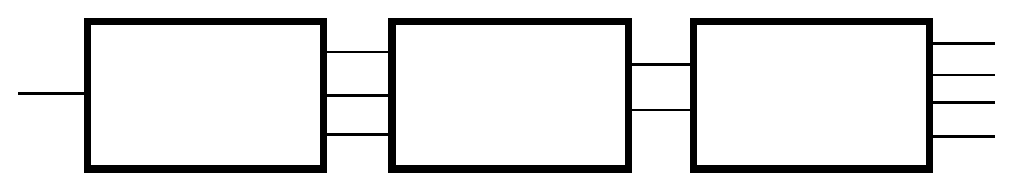
\includegraphics[scale=.5]{./composition/pictures/diagram1.eps}

The input ``\texttt{a ; b c}'' given component input/outputs as: \texttt{a} 3$\rightarrow$3, \texttt{b} 1$\rightarrow$3, and \texttt{c} 6$\rightarrow$2.
Generates the diagram:

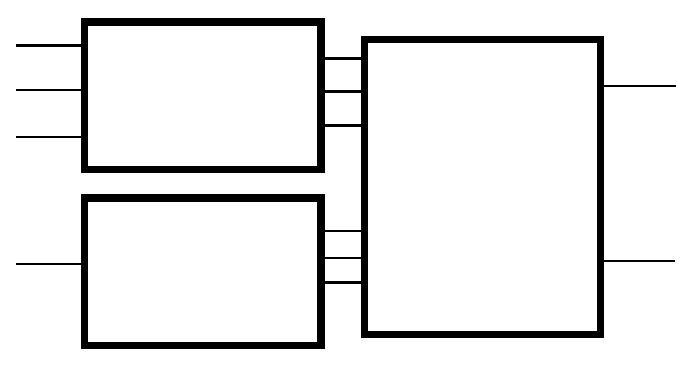
\includegraphics[scale=.5]{./composition/pictures/diagram2.eps}

Note that there are no parenthesis in Dolly's language and thus no groupings that aren't immediate left to right.
This means that some descriptions are invalid, for instance if a component on the left does not have enough input wires for a component on the right.
Dolly will never give you a description that doesn't have two components on either side of a special symbol or a name of a component that doesn't exist, but she might mess up the wire input/outputs.
She's only human after all!

Dolly wants to know what the number of input wires and the number of output wires are for a given description of a component chain.
She's contracted to you to process her descriptions in batch every time she's accumulated enough interesting ones to have them checked.
Because she has a tendency to mess up, she wants you to just output ``-1'' if her description is invalid.
\end{problem}

\newpage

\begin{formalin}
The first line of input consists of two integers, $n$ ($1 \leq n \leq 26$), the number of components, and $q$, ($1 \leq q \leq 1000$) the number of queries.
The next $n$ lines consist of a lowercase english letter, $x$, the name of a component, and two integers, $a$, and $b$, ($1 \leq a, b \leq 100$) the number of input/output wires for the component.
The following $q$ lines consists of an integer $m$, and then $m$ characters which are either lowercase english letters or the character ``\texttt{;}'', describing the component chain.
\end{formalin}

\begin{formalout}
For each query output either two integers, the final input/output configuration for the component chain, or the integer $-1$, if the description is invalid.
\end{formalout}

\begin{datain}
4 3
f 2 3
g 3 1
h 1 2
k 4 1
3 f g h
5 f ; g k h 
3 f k h
\end{datain}

\begin{dataout}
2 2
5 2
-1
\end{dataout}
